\iffalse
\def\mytitle{MATRICES USING PYTHON}
\def\myauthor{Ballepu Dheeraj Kumar}
\def\contact{dheeraj.ballepu@gmail.com}
\def\mymodule{Future Wireless Communication (FWC)}
\documentclass[10pt, a4paper]{article}
\usepackage[a4paper,outer=1.5cm,inner=1.5cm,top=1.75cm,bottom=1.5cm]{geometry}
\twocolumn
\usepackage{graphicx}
\graphicspath{{./images/}}
\usepackage[colorlinks,linkcolor={black},citecolor={blue!80!black},urlcolor={blue!80!black}]{hyperref}
\usepackage[parfill]{parskip}
\usepackage{lmodern}
\usepackage{amsmath,amsfonts,amssymb,amsthm}
\usepackage{tikz}
	\usepackage{physics}
%\documentclass[tikz, border=2mm]{standalone}
\usepackage{karnaugh-map}
%\documentclass{article}
\usepackage{tabularx}
\usepackage{circuitikz}
\usetikzlibrary{calc}
\usepackage{amsmath}
\usepackage{amssymb}
\renewcommand*\familydefault{\sfdefault}
\usepackage{watermark}
\usepackage{lipsum}
\usepackage{xcolor}
\usepackage{listings}
\usepackage{float}
\usepackage{titlesec}
\providecommand{\norm}[1]{\left\lVert#1\right\rVert}
\providecommand{\sbrak}[1]{\ensuremath{{}\left[#1\right]}}
\providecommand{\lsbrak}[1]{\ensuremath{{}\left[#1\right.}}
\providecommand{\rsbrak}[1]{\ensuremath{{}\left.#1\right]}}
\providecommand{\brak}[1]{\ensuremath{\left(#1\right)}}
\providecommand{\lbrak}[1]{\ensuremath{\left(#1\right.}}
\providecommand{\rbrak}[1]{\ensuremath{\left.#1\right)}}
\providecommand{\cbrak}[1]{\ensuremath{\left\{#1\right\}}}
\providecommand{\lcbrak}[1]{\ensuremath{\left\{#1\right.}}
\providecommand{\rcbrak}[1]{\ensuremath{\left.#1\right\}}}
\newcommand{\myvec}[1]{\ensuremath{\begin{pmatrix}#1\end{pmatrix}}}
\let\vec\mathbf
\providecommand{\mtx}[1]{\mathbf{#1}}
\titlespacing{\subsection}{1pt}{\parskip}{3pt}
\titlespacing{\subsubsection}{0pt}{\parskip}{-\parskip}
\titlespacing{\paragraph}{0pt}{\parskip}{\parskip}
\newcommand{\figuremacro}[5]

\begin{document}

\title{\mytitle}
\author{\myauthor\hspace{1em}\\\contact\\FWC22008\hspace{6.5em}IITH\hspace{0.5em}\mymodule\hspace{6em}ASSIGN-4}
\date{}
	\maketitle
		
	\tableofcontents
\vspace{5mm}
   \section{Problem}
   \fi
$ABCD$ is a rhombus. Show that the diagonal $AC$ bisects angle $A$ as well as angle $C$ and diagonal $BD$ bisects angle $B$ as well as angle $D$. 
\\
\solution
\iffalse
}
   \section{Solution}
   \textbf{Theory:}\\

   Given  ABCD is a rhombus \\ 
  

\textbf{To Prove:} Diagonals bisects angles\\
\fi
%
For the rhombus in Fig. 
		\ref{fig:9/8/1/7},
 	\begin{figure}
		\centering
 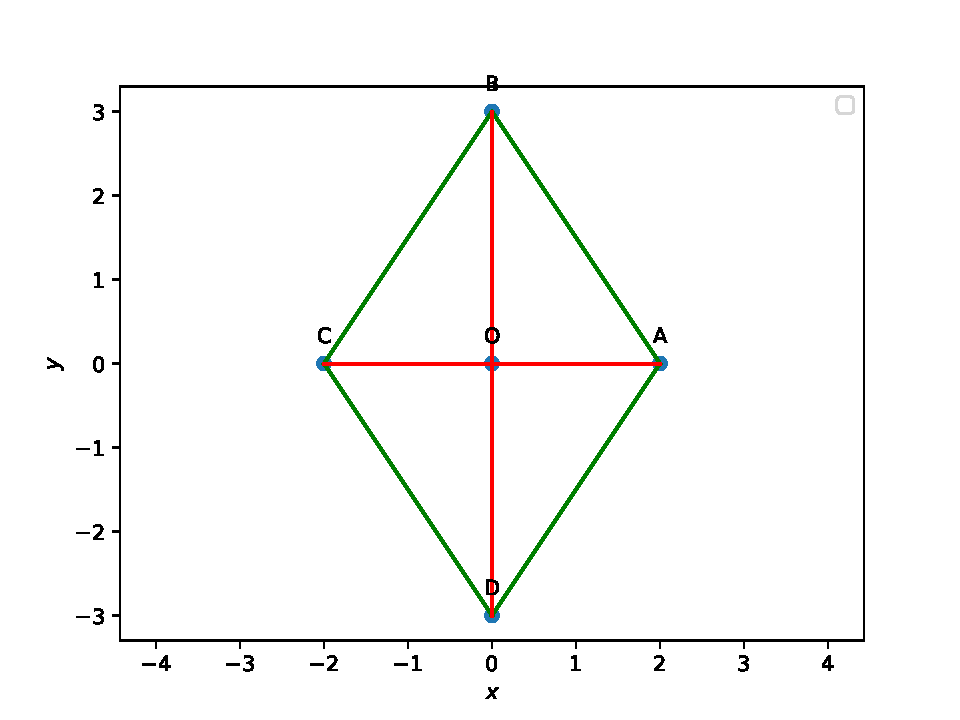
\includegraphics[width=\columnwidth]{chapters/9/8/1/7/figs/fig5.pdf} 
		\caption{}
		\label{fig:9/8/1/7}
  	\end{figure}
\begin{align}
		\label{eq:9/8/1/7}
		\begin{split}
	\norm{\vec{A}-\vec{B}}&=\norm{\vec{A}-\vec{D}}
\\
	\vec{A}-\vec{B}&=\vec{D}-\vec{C}
		\end{split}
\end{align}
From 
    \eqref{eq:angle2d},
\begin{align}
		\begin{split}
	\cos \angle{BAC}
	&= \frac{(\vec{A}-\vec{B})^T(\vec{A}-\vec{C})}{\norm{\vec{A}-\vec{B}}\norm{\vec{A}-\vec{C}}}
	\\
\cos	\angle{DAC}
	 &= \frac{(\vec{C}-\vec{D})^T(\vec{C}-\vec{A})}{\norm{\vec{C}-\vec{D}}\norm{\vec{C}-\vec{A}}}
		\end{split}
	 \label{eq:9/8/1/8/cang}
%
\end{align}
From 
		\eqref{eq:9/8/1/7}
and
	 \eqref{eq:9/8/1/8/cang}, 
%
	 we obtain
\begin{align}
		\begin{split}
	\cos \angle{BAC}
	=\cos \angle{DAC}
		\end{split}
\end{align}
Thus, $AC$ bisects $\angle A$.  Similarly, the remaining results can be proved.
